\chapter{Bildverarbeitung}

Die Bildverarbeitung besteht im Wesentlichen aus der Generierung von einzelnen Videoframes im RGB565 – Bitmap Format, welche optisch den Anforderungen aus \textbf{Kapitel X} entsprechen müssen. Die einzelnen Videoframes werden von der Schnittstelle \textbf{IFrameProvider} empfangen und nach der Verarbeitung an die Schnittstelle \textbf{FrameViewer} zur Darstellung auf dem Display des Smartphones weitergereicht.
\\
\\
Im ersten Ansatz, der verfolgt wurde, benötigte es eine Konvertierung als Vorverarbeitung der einzelnen Frames in den RGB Farbraum (siehe Kapitel \ref{YUV_RGBKonvert}). Diese Vorverarbeitung wurde im späteren Verlauf überflüssig, da das Übertragungsformat der Videoframes aufgrund der in \textbf{Kapitel X} aufgelisteten Gründen geändert wurde. Der Vollständigkeit halber wird eben genannte Konvertierung hier trotzdem erläutert.
\\
\\
Es wurde davon ausgegangen, dass die Schnittstelle \textbf{IFrameProcessor} Byte-Streams im Format NV12 (YUV420) erhält, welche zur weiteren Verarbeitung zunächst in den RGB Farbraum überführt werden mussten, um dann als Bitmap-Objekte weiterverarbeitet werden zu können. Die NV12 Byte-Streams liegen im YUV-Farbmodell (siehe Kapitel \ref{YUV_RGBKonvert}) vor. 
\\
\\
Die Methode convertNv12ToBmp(...) (siehe Abbildung \ref{fig:NV12_to_BMP})nimmt ein eindimensionales Byte-Array, welches ein Frame im NV12-Format repräsentiert, entgegen. Die Methode benötigt zusätzlich noch die Höhe und Breite des Frames in Pixeln, um die Positionen der für ein Ausgabepixel relevanten Y, U und V Werte im Array bestimmen zu können. Innerhalb der for-Schleife werden für jedes einzelne Ergebnis-Pixel die in Kapitel \ref{YUV} Luminanz- und Chrominanz-Werte aus dem Array ermittelt und an die Methode convertYUVtoRGB(...) übergeben. Ergebnis dieser Methode ist ein Array aus Integer-Werten, welche jeweils die Farbe eines Pixels repräsentieren. Mit Hilfe dieses Arrays kann anschließend mit der Methode createBitmap(...) der Klasse Bitmap aus dem Android SDK ein Bitmap-Objekt erzeugt werden. 
\clearpage
\begin{figure}[h]
	\centering
	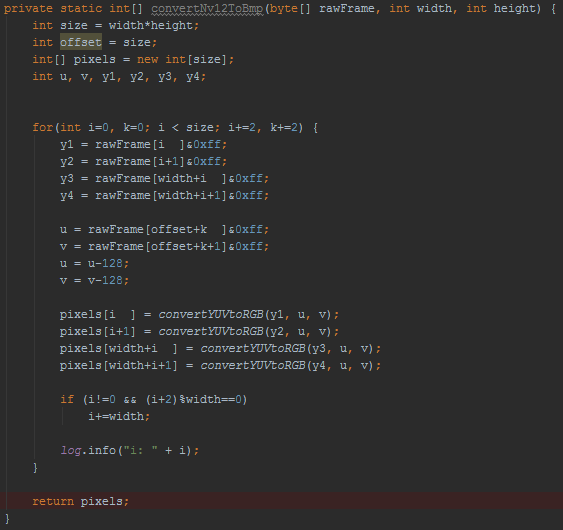
\includegraphics[width=0.9\textwidth]{Bilder/Bildverarbeitung/NV12_to_BMP.PNG}
	\caption{Methode zur Überführung eines Byte-Arrays im NV12-Format in ein Bitmap-Objekt}
	\label{fig:NV12_to_BMP}
\end{figure}

~\\
Die in Abbildung \ref{fig:YUV_to_RGB} gezeigte Methode convertYUVtoRGB(...) übernimmt gemäß der Formeln aus Kapitel \ref{YUV_RGBKonvert} die Berechnung der R, G und B Werte eines Pixels des Ergebnis-Frames. Aus diesen drei Werten wird anschließend ein Integer berechnet, welcher dann allein die Farbe des Pixels repräsentiert.
\clearpage
\begin{figure}[h]
	\centering
	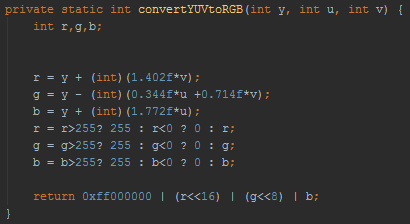
\includegraphics[width=0.7\textwidth]{Bilder/Bildverarbeitung/convert_1_Pixel.PNG}
	\caption{Methode zur Umrechnung eines Pixels aus dem YUV-Farbraum in den RGB-Farbraum}
	\label{fig:YUV_to_RGB}
\end{figure}

~\\
Wie bereits weiter oben erwähnt, wurde die eben beschriebene Konvertierung obsolet, da der FrameProcessor-Schnittstelle aus in \textbf{Kapitel X} genannten Gründen direkt die einzelnen Videoframes als Bitmap-Objekte im RGB565 Format geliefert bekommt. Diese Frames beinhalten das unveränderte Bildmaterial des Ultraschallgeräts, wie es auf dessen Monitor angezeigt wird. Da nicht alle Komponenten des Bildes relevant für die Erfüllung der in \textbf{Kapitel X} beschriebenen Anforderungen sind, erfolgt zunächst eine Auswahl der relevanten Ausschnitte des Bildes, um diese anschließend gemäß der Konzeptzeichnung (siehe Abbildung \ref{fig:Ausgabeframe}) neu anzuordnen. 

\begin{figure}[h]
	\centering
	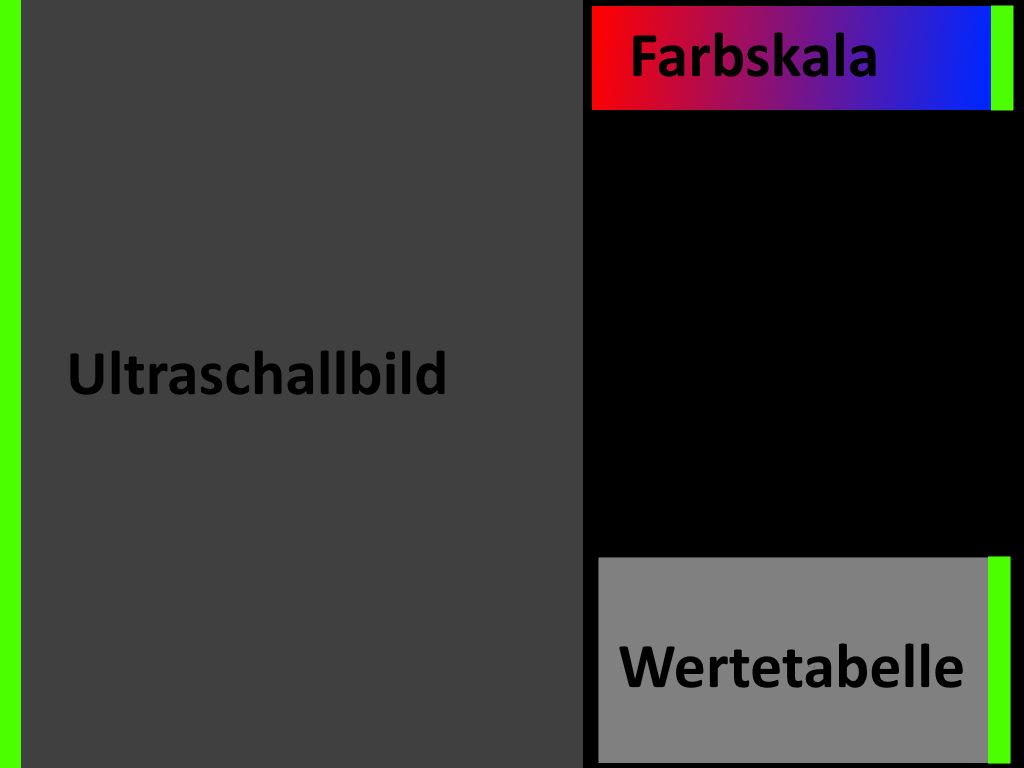
\includegraphics[width=0.5\textwidth]{Bilder/Bildverarbeitung/Konzept_Endframe.PNG}
	\caption{Konzeptzeichnung Ausgabeframe}
	\label{fig:Ausgabeframe}
\end{figure}

~\\
Der grüne Rand der einzelnen Komponenten in der Konzeptzeichnung (Abbildung \ref{fig:Ausgabeframe}) zeigt den oberen Rand dieser im Originalbild. Das Ultraschallbild wird also entsprechend um 270° und die Farbskala und Wertetabelle um 90° gedreht dargestellt. Zu beachten ist, dass die Ausgabeframes auf dem Display des Smartphones vertikal mit dem Ultraschallbild zum Teilerspiegel zeigend dargestellt werden. Diese Anordnung ermöglicht eine Darstellung des Ultraschallbildes in der Breite des Schallkopfes und eine leichte Lesbarkeit der Wertetabelle und Farbskala.
\\
\\
Abbildung \ref{fig:extractUltrasonicScan} zeigt beispielhaft für das Ausschneiden der für das Ausgabebild relevanten Komponenten die Methode extractUltrasonicScan(). Da sich das Ultraschallbild an fester Stelle im Originalvideo befindet, konnten feste Werte für dieses ermittelt und in der Methode verwendet werden. Aus dem ausgeschnittenen Rechteck wird dann ein Bitmap-Objekt der Größe dessen generiert.

\begin{figure}[h]
	\centering
	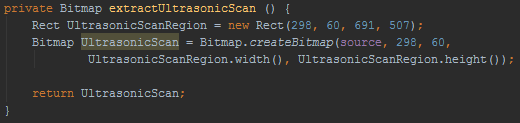
\includegraphics[width=0.9\textwidth]{Bilder/Bildverarbeitung/extractUltrasonicScan.PNG}
	\caption{Methode zum Ausschneiden des Ultraschallbildbereichs aus dem Originalframe}
	\label{fig:extractUltrasonicScan}
\end{figure}

~\\
Die nachfolgend abgebildete Methode buildFinalFrame() (Abbildung \ref{fig:buildFinalFrame}) baut die einzelnen Komponenten, welche mit den Methoden extractUltrasonicScan(), extractColorScale() und extractValues() extrahiert werden, zu einem Frame gemäß Abbildung \ref{fig:Ausgabeframe} zusammen. Hierzu werden zunächst zwei Rotationsmatrizen erzeugt, eine die eine Rotation um 270° und eine, die eine Rotation um 90° vollzieht. Mit Hilfe dieser Matrizen werden anschließend die drei Komponenten rotiert und in neuen Bitmap-Objekten zwischengespeichert. Für das Bitmap-Objekt result werden die Konfigurationen des Quellobjekts übernommen. Anschließend wird es einem Canvas-Objekt übergeben, auf dem dann die drei vorverarbeiteten Komponenten angeordnet werden. Hierfür wird noch eine Skalierung des Ultraschallbildobjekts vorgenommen, sodass dies die volle Höhe des Ausgabeframes als Breite beansprucht (siehe Abbildung \ref{fig:Ausgabeframe}).
\clearpage
\begin{figure}[h]
	\centering
	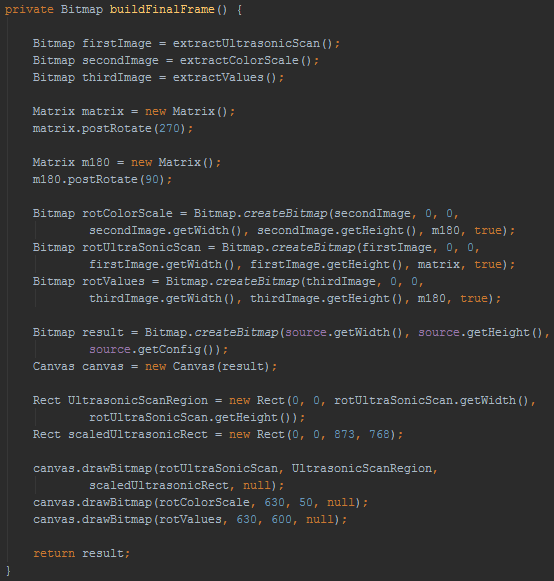
\includegraphics[width=1\textwidth]{Bilder/Bildverarbeitung/buildFinalFrame.PNG}
	\caption{Methode zum Zusammenstellen des Ausgabeframes}
	\label{fig:buildFinalFrame}
\end{figure}
\clearpage
~\\
Um die Unschönheit zu vermeiden, dass bereits vor dem Schallen Frames der Auswahlfenster der SonoScape-Software verarbeitet und zur Anzeige auf das Display des Smartphones gebracht werden, wurde eine Methode geschrieben, welche überprüft ob die SonoScape-Software in den Schall-Modus gewechselt ist. Diese Überprüfung geschieht simpel über einen Farbvergleich von Pixeln. Es wurden Pixel an Positionen gewählt, bei denen davon auszugehen ist, dass ihre Farbe schwarz ist, solange sich die SonoScape-Software im Schall-Modus befindet.  
\\
\\
Zum isolierten Testen der Bildverarbeitung im FrameProcessor wurde eine Testklasse FrameProcessorImplTest geschrieben, welche einzelne Testframes als BIN-Dateien, die zuvor mit dem Ultraschallgerät aufgenommen wurden, aus dem SD-Kartenspeicher des Smartphones (oder des Emulators) lädt und diese zum Verarbeiten an die FrameProcessor-Schnittstelle weiterleitet. Für die Evaluierung der Bildverarbeitung wurden die bearbeiteten Frames anschließend als PNG-Dateien wieder in den SD-Kartenspeicher geschrieben. 
\\
Um Testdateien in den SD-Kartenspeicher des AndroidStudio-Emulators (siehe Kapitel \ref{Android}) zu schreiben, bzw. sie aus diesem auszulesen, wurden folgende Befehle über die AndroidStudio-Konsole eingegeben:
\\
Schreiben: \textit{adb push path/yourfile.xxx /sdcard/yourfile.xxx}
\\
Lesen: \textit{adb pull /sdcard/yourfile.xxx /path/yourfile.xxx}
\\
Damit die FrameProcessor-Schnittstelle überhaupt angesprochen werden kann, musste für die Testklasse die Methode loadRGBFile() (Abbildung \ref{fig:BIN_to_Bitmap}) implementiert werden, die aus einer BIN-Datei, die ein Frame im RGB565-Format enthält, ausliest und in ein Bitmap-Objekt schreibt. 

\clearpage
\begin{figure}[h]
	\centering
	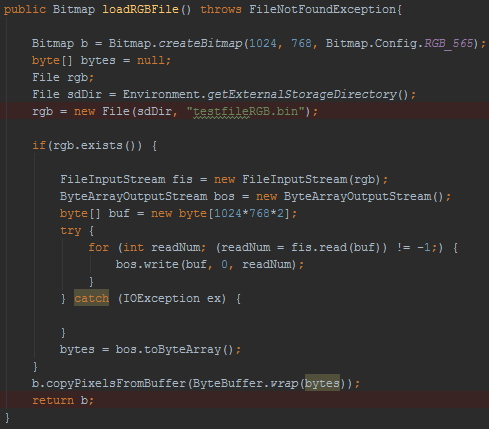
\includegraphics[width=0.8\textwidth]{Bilder/Bildverarbeitung/BIN_to_Bitmap.PNG}
	\caption{Methode zum Einlesen einer BIN-Datei im RGB565-Format zu Testzwecken}
	\label{fig:BIN_to_Bitmap}
\end{figure}